\documentclass[mathserif,notes]{beamer} % Math 298 Fall 2014
\usepackage{pdfsync} % works only on TeXShop, comment otherwise
\usepackage{pgf}
\usepackage{multimedia} % to embed movies in the PDF file
\usepackage{xcolor}
\usepackage{graphicx}
\usepackage{comment}
\usepackage{pgfpages}
\usepackage{topcapt}
\usepackage{booktabs}
\usepackage{mathtools}

% for the tikz pictures
\usepackage{geometry}
%\geometry{hmargin=1cm,vmargin=1cm}
\usepackage{tikz}
\def\width{5}
\def\hauteur{5}
\mode<presentation>
{
  \usetheme{Madrid}   %  \usetheme{Warsaw}
  % Note: this next command makes nice slides, but Adobe doesn't like it (you get blank pages)
  \setbeamertemplate{background canvas}[vertical shading][bottom=white,top=structure.fg!15]
  %\setbeamertemplate{footline}{\pgfuseimage{UCM-logo}}

  %\usecolortheme{seahorse}
  \usecolortheme{beaver}
 % \setbeamercovered{transparent}
}
%\usepackage[T1]{fontenc}
% For printing purposes only
%\pgfpagesuselayout{2 on 1}[letterpaper,border shrink=5mm,portrait]
\pgfpagesuselayout{resize to}[letterpaper,border shrink=5mm,landscape]  % print out full size on paper

\usepackage{amssymb,amsmath}
\hypersetup{%
 pdftitle={Math298 Lecture 6},
 pdfauthor={Juan Meza(UC Merced)},
 pdfsubject={Fundamental Concepts in Computational and Applied Mathematics},
 pdfkeywords={spectral methods, FFT, DFT}
 }
 
\title[Math 298 Lecture 6: Spectral Methods]{Fundamental Concepts in \\ Computational and Applied Mathematics}  \subtitle{}
\author[Juan Meza]{Juan Meza \\ School of Natural Sciences \\ University of California, Merced}
\date[Fall 2014]{Fall 2014}
\institute[UC Merced]

%\pgfdeclareimage[height=0.35cm]{UCM-logo}{UCM-logo}
% \logo{\pgfuseimage{UCM-logo}}

%% figures






% Common abbreviations
% (Remember to put '\ ' after if an interword space is
%  desired rather than end-of-sentence space. Same for '.etc)' ).
\newcommand{\eg}{{\em e.g.}}		% e.g.
\newcommand{\ie}{{\em i.e.}}		% i.e.
\newcommand{\etc}{{\em etc.}}		% etc.
\newcommand{\vs}{{\em vs.}}		% vs.
\newcommand{\remark}{{\color{red} Remark:} }


\newcommand {\DS} {\displaystyle}
\newcommand{\eref}[1]{{\rm{(\ref{#1})}}}
\newcommand{\tref}[1]{{\rm{\ref{#1}}}}


\def\frechet{Fr\'echet\ }
\def\more{Mor\'e\ }
\def\fl{{\sf fl}}
\def\flop{{\sf flop} }
\def\flops{{\sf flops} }
\def\matlab{{\sc Matlab} }
\def\Matlab{\matlab}

\def\bigO{\mathcal{O}}

% Mathematical Symbols

\newcommand{\deq}{\raisebox{0pt}[1ex][0pt]{$\stackrel{\scriptscriptstyle{\rm def}}{{}={}}$}}

\newcommand {\half} {\mbox{$\frac{1}{2}$}}  %machine epsilon
\newcommand{\set}[2]{\left\{ #1 \;:\; #2 \right\}}

\newcommand {\macheps} {\mathbf{\epsilon}}  %machine epsilon
\newcommand {\real} {\mathbb{R}}
\newcommand {\nat} {\mathbb{N}}
\newcommand {\compl} {\mathbb{C}}
\newcommand {\diag} {{\mbox{diag}}}
\newcommand {\meas} {{\mbox{meas}}}
\newcommand {\mspan} {{\mbox{span}}}

\newcommand {\pdx} {\frac{\partial}{\partial x}}
\newcommand {\pdt} {\frac{\partial}{\partial t}}
\newcommand {\pdxx} {\frac{\partial^2}{\partial x^2}}
\newcommand {\dx} {\frac{d}{d x}}
\newcommand {\dt} {\frac{d}{d t}}
\newcommand {\dxx} {\frac{d^2}{d x^2}}

\newcommand {\bA} {\mbox{\boldmath $A$}}
\newcommand {\bB} {\mbox{\boldmath $B$}}
\newcommand {\bF} {\mbox{\boldmath $F$}}
\newcommand {\bI} {\mbox{\boldmath $I$}}
\newcommand {\bP} {\mbox{\boldmath $P$}}
\newcommand {\bY} {\mbox{\boldmath $Y$}}
\newcommand {\bZ} {\mbox{\boldmath $Z$}}
\newcommand {\ba} {\mbox{\boldmath $a$}}
\newcommand {\bb} {\mbox{\boldmath $b$}}
\newcommand {\bd} {\mbox{\boldmath $d$}}
\newcommand {\bff}{\mbox{\boldmath $f$}}
\newcommand {\bk} {\mbox{\boldmath $k$}}
\newcommand {\bp} {\mbox{\boldmath $p$}}
\newcommand {\bs} {\mbox{\boldmath $s$}}
\newcommand {\bu} {\mbox{\boldmath $u$}}
\newcommand {\bv} {\mbox{\boldmath $v$}}
\newcommand {\bw} {\mbox{\boldmath $w$}}
\newcommand {\bx} {\mbox{\boldmath $x$}}
\newcommand {\by} {\mbox{\boldmath $y$}}
\newcommand {\bz} {\mbox{\boldmath $z$}}
\newcommand {\blambda} {\mbox{\boldmath $\lambda$}}
\newcommand {\btau} {\mbox{\boldmath $\tau$}}

%
% JCM Quantum Chemistry commands
%
\newcommand{\bra}[1]{\langle #1|}
\newcommand{\ket}[1]{|#1\rangle}
\newcommand{\braket}[2]{\langle #1|#2\rangle}
% Example of usage
%\[
%\ket{\Psi}=\sum_{i}\ket{\phi_i}\braket{\phi_i}{\Psi}
%\]

%
% Other symbols
%
\newcommand {\grad}{\nabla}
\newcommand {\hess}{\nabla^2}
\newcommand {\condA}{\kappa(A)}

\newtheorem{algorithm}{Algorithm}

%

% \boxfig{pos}{wid}{text}:  A figure with a box around it
%
% pos	the usual figure placement arg: eg. htbp
% wid	the width of the figure, in some units: eg. 5in
% text	the contents of the figure, including picture/caption/label/etc
%
\newlength{\boxwidth}
\newcommand{\boxfigure}[3]{
	\begin{figure}[#1]
		\setlength{\boxwidth}{#2}
		\addtolength{\boxwidth}{.1in}

		\centering
		\framebox[\boxwidth]{
			\begin{minipage}{#2}
			#3
			\end{minipage}
		}
	\end{figure}  
}

% use \fullboxwidth for arg 2 of boxfigure to get box of size \textwidth


% \boxalg{pos}{text}:  An algorithm with a box around it
%
% title  the name of the algorithm
% text   the contents of the figure, including picture/caption/label/etc
%
\newcommand{\boxalg}[2]{
            \setlength{\boxwidth}{\fullboxwidth}
            \addtolength{\boxwidth}{.1in}
            \vspace{2ex}
            \framebox[\boxwidth][#1]{
                    \vspace{1ex}
                    \begin{minipage}{\fullinboxwidth}
                        #2
                    \end{minipage}
                    \vspace{1ex}
            }
            \vspace{2ex}
}






% see above
\newlength{\fullboxwidth}
\setlength{\fullboxwidth}{\textwidth}
\addtolength{\fullboxwidth}{-0.5in}

\newlength{\fullinboxwidth}
\setlength{\fullinboxwidth}{\fullboxwidth}
\addtolength{\fullinboxwidth}{-0.5in}






\definecolor{navy}{RGB}{0,0,128}
\definecolor{forestgreen}{RGB}{34,139,34}
\definecolor{mylightsteelblue}{RGB}{176,196,222}
\definecolor{mylightcyan}{RGB}{180,255,255}
\definecolor{mypaleturquoise}{RGB}{175,238,238}
\definecolor{mylightgoldenrod}{RGB}{250,250,210}
\definecolor{mylightyellow}{RGB}{255,255,224}
\definecolor{mylightsalmon}{RGB}{255,160,122}

\setbeamercolor{blacklightsteelblue}{fg=black,bg=mylightsteelblue}
\setbeamercolor{blackpaleturquoise}{fg=black,bg=mypaleturquoise}
\setbeamercolor{blacklightcyan}{fg=black,bg=mylightcyan}
\setbeamercolor{blacklightgoldenrod}{fg=black,bg=mylightgoldenrod}
\setbeamercolor{blacklightyellow}{fg=black,bg=mylightyellow}
\setbeamercolor{blacklightsalmon}{fg=black,bg=mylightsalmon}
\setbeamercolor{blackcyan}{fg=black,bg=cyan}




\begin{document}

%%%%%%%%%%%%%%%%%%%%%%%%%%%%%%%%%%%%%%%%%%%%%
\frame{

\titlepage

} % end frame

\section{Introduction}
%%%%%%%%%%%%%%%%%%%%%%%%%%%%%%%%%%%%%%%%%%%%%
\frame{\frametitle{Spectral methods}

\begin{itemize}
\item Up until now we've been concerned with solving problems in the temporal \& spatial domains
\item Spectral methods transform the problem and work in the frequency domain (sometimes called phase space).
\item Particularly useful in problems that have periodicity or infinite domains
\item Still useful if that's not the case 
\end{itemize}
} % end frame

%%%%%%%%%%%%%%%%%%%%%%%%%%%%%%%%%%%%%%%%%%%%%
\frame{\frametitle{Motivation}

\begin{itemize}
\item Consider the case of differentiation of a function
\item One possibility is finite differences
\item Another general idea: Interpolate the function of interest by a polynomial and then take derivative of polynomial
\item This idea leads to the notion of a differentiation matrix
\end{itemize}

} % end frame


%%%%%%%%%%%%%%%%%%%%%%%%%%%%%%%%%%%%%%%%%%%%%
\frame{\frametitle{Motivation}

\begin{itemize}
\item Consider  a periodic function $u(x)$ in 1D, on an equally spaced grid 
\item $h$ is the spatial discretization
\item $u(0) = u(N)$
\vspace{.25in}

\end{itemize}
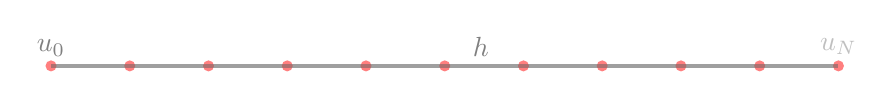
\begin{tikzpicture}[x=1cm, y=1cm, semitransparent]
%\draw[step=1mm, line width=0.1mm, black!30!white] (0,0) grid (\width,\hauteur);
%\draw[step=5mm, line width=0.2mm, black!40!white] (0,0) grid (\width,\hauteur);
\draw[step=5cm, line width=0.5mm, black!50!white] (0,0) grid (10,0);
%\draw[step=1cm, line width=0.5mm, black!50!white] (1,1) grid (10,0);


    \coordinate (u0) at (0,0)     node[above]  {$u_0$};  
    \coordinate (u1) at (1,0);
    \coordinate (u2) at (2,0);
    \coordinate (u3) at (3,0);
    \coordinate (u4) at (4,0);
    \coordinate (u5) at (5,0);
    \coordinate (u6) at (6,0);
    \coordinate (u7) at (7,0);
    \coordinate (u8) at (8,0);
    \coordinate (u9) at (9,0);
    \coordinate (u10) at (10,0);
    \fill[red] (u0) circle (2pt);
    \fill[red] (u1) circle (2pt);
    \fill[red] (u2) circle (2pt);
    \fill[red] (u3) circle (2pt);
    \fill[red] (u4) circle (2pt);
     \fill[red] (u5) circle (2pt) node[ above right ] {$\ \ {\color{black} h}$};
     \fill[red] (u6) circle (2pt);
     \fill[red] (u7) circle (2pt);
     \fill[red] (u8) circle (2pt);    
     \fill[red] (u9) circle (2pt);
     \fill[red] (u10) circle (2pt);

\draw[step=1cm, line width=0.5mm, black!50!white] (0,0) grid (10,0)     node[above] {$u_N$};;

                
\end{tikzpicture}
$$
{w^{\prime}}(x) = \frac{u(x_{j+1}) - u(x_{j-1})}{2h}
$$
} % end frame


%%%%%%%%%%%%%%%%%%%%%%%%%%%%%%%%%%%%%%%%%%%%%
\frame{\frametitle{Differentiation Matrix}

\begin{itemize}

\item A second order method can be given by the following matrix
\end{itemize}

$$
D= \begin{bmatrix*}[r]
0          & 1/2        &   &   &  & -1/2 \\
-1/2      &     0       &  1/2 &  & &   \\
          & -1/2      &  0 & 1/2 &   &    \\
 &            &  -1/2 &  0 & 1/2 &    \\
          &          &  &  -1/2 & 0   &  1/2    \\
1/2       &           &   & & -1/2     &   0 \\
\end{bmatrix*}
$$
The derivative is given by $w = \frac{1}{h} D \cdot u$
\vspace{.25in}

{\color{red} Recall:}  This matrix is skew-symmetrix, Toeplitz (diagonal-constant), and circulant!   \\

} % end frame

%%%%%%%%%%%%%%%%%%%%%%%%%%%%%%%%%%%%%%%%%%%%%
\frame{\frametitle{Spectral Method}

General Principle
\begin{itemize}
\item Generate a high-order interpolant of your function, e.g. trigonometric polynomial
\item Take the derivative of the interpolant
\item Substitute this in your differential equation

\end{itemize}

} % end frame

\section{Discrete Fourier Transform}
%%%%%%%%%%%%%%%%%%%%%%%%%%%%%%%%%%%%%%%%%%%%%
\frame{\frametitle{Discrete Fourier Transform}

Suppose we have $X \in R^N$. \\
Then the DFT of $X$ denoted by $\hat{X}(k) $ is given by
\begin{equation}
\hat{X}(k) = \sum_{j=0}^{N-1} X(j) W_{N}^{jk}, \label{eq:DFT}
\end{equation}
where
$$
W_{N}^{jk} = \exp \left ( \frac{ -2 \pi i j k}{N} \right ),
$$
which can also be viewed as a matrix-vector multiply $F_N \cdot X$, where
$$
F_N = W_N^{jk}
$$
and the $k$ are called {\em wave numbers}.

} % end frame

%%%%%%%%%%%%%%%%%%%%%%%%%%%%%%%%%%%%%%%%%%%%%
\frame{\frametitle{Example: N = 2, 4}
Let $\omega =  \exp \left ( \frac{- 2 \pi i }{N} \right ).$ \\
\vspace{.25in}
$N = 2$
$$
F_2 = 
\begin{bmatrix*}[r]
1   & 1                 \\
1   & -1      
\end{bmatrix*}, 
$$
$N= 4$
$$
F_4 = 
\begin{bmatrix*}[r]
1   & 1                  &  1                 & 1 \\
1   &  \omega       &  \omega^{2} & \omega^{3}  \\
1   &  \omega^{2} &  \omega^{4} & \omega^{6}  \\
1   &  \omega^{3}  &  \omega^{6} & \omega^{9}  \\
\end{bmatrix*} = 
\begin{bmatrix*}[r]
1   &  1     &  1  & 1 \\
1   & -i      &  -1 & i  \\
1   & -1 &  1& -1  \\
1   &  i  &  -1 & -i \\
\end{bmatrix*}.
$$
} % end frame

%%%%%%%%%%%%%%%%%%%%%%%%%%%%%%%%%%%%%%%%%%%%%
\frame{\frametitle{Key Idea}
One can permute the columns of $F_4$ so that 
$$
F_4 \Pi_{4} = \left [
\begin{array}{r r | r r}
1   &  1     &  1  & 1 \\
1   & -1    &  -i & i  \\
\hline
1   & 1 &   -1& -1  \\
1   & -1  &  i & -i \\
\end{array} \right ], \qquad 
\Pi_4 = \begin{bmatrix}
1   &  0     &  0  & 0 \\
0    & 0      &  1 & 0  \\
0   &  1 &  0& 0  \\
0   &  0  &  0 & 1 \\
\end{bmatrix}
$$
which is just $F_4$ with even-indexed columns ordered first.
} % end frame

%%%%%%%%%%%%%%%%%%%%%%%%%%%%%%%%%%%%%%%%%%%%%
\frame{\frametitle{Key Idea}
Now notice that for $N =4$
$$
F_4 \Pi_{4} = 
\begin{bmatrix*}[r]
F_2   & \Omega_2 F_2               \\
F_2  & -  \Omega_2 F_2   
   
\end{bmatrix*}, 
$$
where
$$
\Omega_{2} = 
\begin{bmatrix*}[r]
 1  & 0  \\
0  & -i    
\end{bmatrix*}, 
$$
in other words, each block of $F_4\Pi_4$ is either $F_2$ or a diagonal scaling of $F_2$ and
$F_2$ is of size $N/2$

} % end frame

%%%%%%%%%%%%%%%%%%%%%%%%%%%%%%%%%%%%%%%%%%%%%
\frame{\frametitle{Some consequences}

\begin{itemize}
\item An $N-$point DFT can be computed from two $N/2-$point DFTs!
\item The complexity of the algorithm can be shown to be $\mathcal{O}(N \log N)$ vs. $\mathcal{O}(N^2)$
\item Spectral methods are highly accurate for smooth functions
\end{itemize}

}% end frame


%%%%%%%%%%%%%%%%%%%%%%%%%%%%%%%%%%%%%%%%%%%%%
\frame{\frametitle{FFT}
Recall

$$
u_j = \sum^N_{k=1} e^{2\pi i j k / N} \cdot w_k , \quad j = 1, \ldots, N. 
$$

\vspace{.25in}
What is the complexity for such an algorithm?
} % end frame

%%%%%%%%%%%%%%%%%%%%%%%%%%%%%%%%%%%%%%%%%%%%%
\frame{\frametitle{Discrete Fourier Transform (DFT) and Fast Fourier Transform (FFT)}

\begin{itemize}
\item The DFT is a natural extension of differentiation to a bounded, periodic grid using Fourier transforms
\item The bounded physical domain implies that the Fourier domain will be discrete, i.e. the wavenumbers, $k$, will be integers
\item The derivative in Fourier space can be computed by multiplying the transform by $ik$
\item The FFT is a fast algorithm for computing the DFT
\end{itemize}

}% end frame


\section{Summary}
%%%%%%%%%%%%%%%%%%%%%%%%%%%%%%%%%%%%%%%%%%%%%
\frame{\frametitle{Summary}

\begin{itemize}
\item Spectral methods work in Fourier (frequency) space
\item The development of the FFT led to many new areas of research and applications
\item Many applications in image processing, computational chemistry, Fast Poisson solvers, etc.
\item Can also be used for non-periodic or non-uniform data, but that's another talk
\end{itemize}

}% end frame

%%%%%%%%%%%%%%%%%%%%%%%%%%%%%%%%%%%%%%%%%%%%%
\begin{frame}[allowframebreaks]
  \frametitle<presentation>{References}    
  \begin{thebibliography}{10}    

     
     \beamertemplatearticlebibitems
      \bibitem{CoTu65}
 James W. Cooley and John W. Tukey.
  \newblock An Algorithm for the Machine Calculation of Complex Fourier Series,
 \newblock Math. Comp. 19, 297-301, 1965. 

  \beamertemplatebookbibitems
 \bibitem{CVL92}
   Charles Van Loan.
    \newblock {\em Computational Frameworks for the Fast Fourier Transform},
   \newblock SIAM,  1992.

     
       \beamertemplatebookbibitems
 \bibitem{Tr2000}
   Lloyd N. Trefethen.
    \newblock {\em Spectral Methods in Matlab},
   \newblock SIAM, 2000.
     \beamertemplatearticlebibitems
  \end{thebibliography}
 \end{frame}
 
\end{document}
